\subsection{Runtime Performance Study}
\label{subsec:runtime-performance-study}
\begin{figure}[htbp]
    \centering
    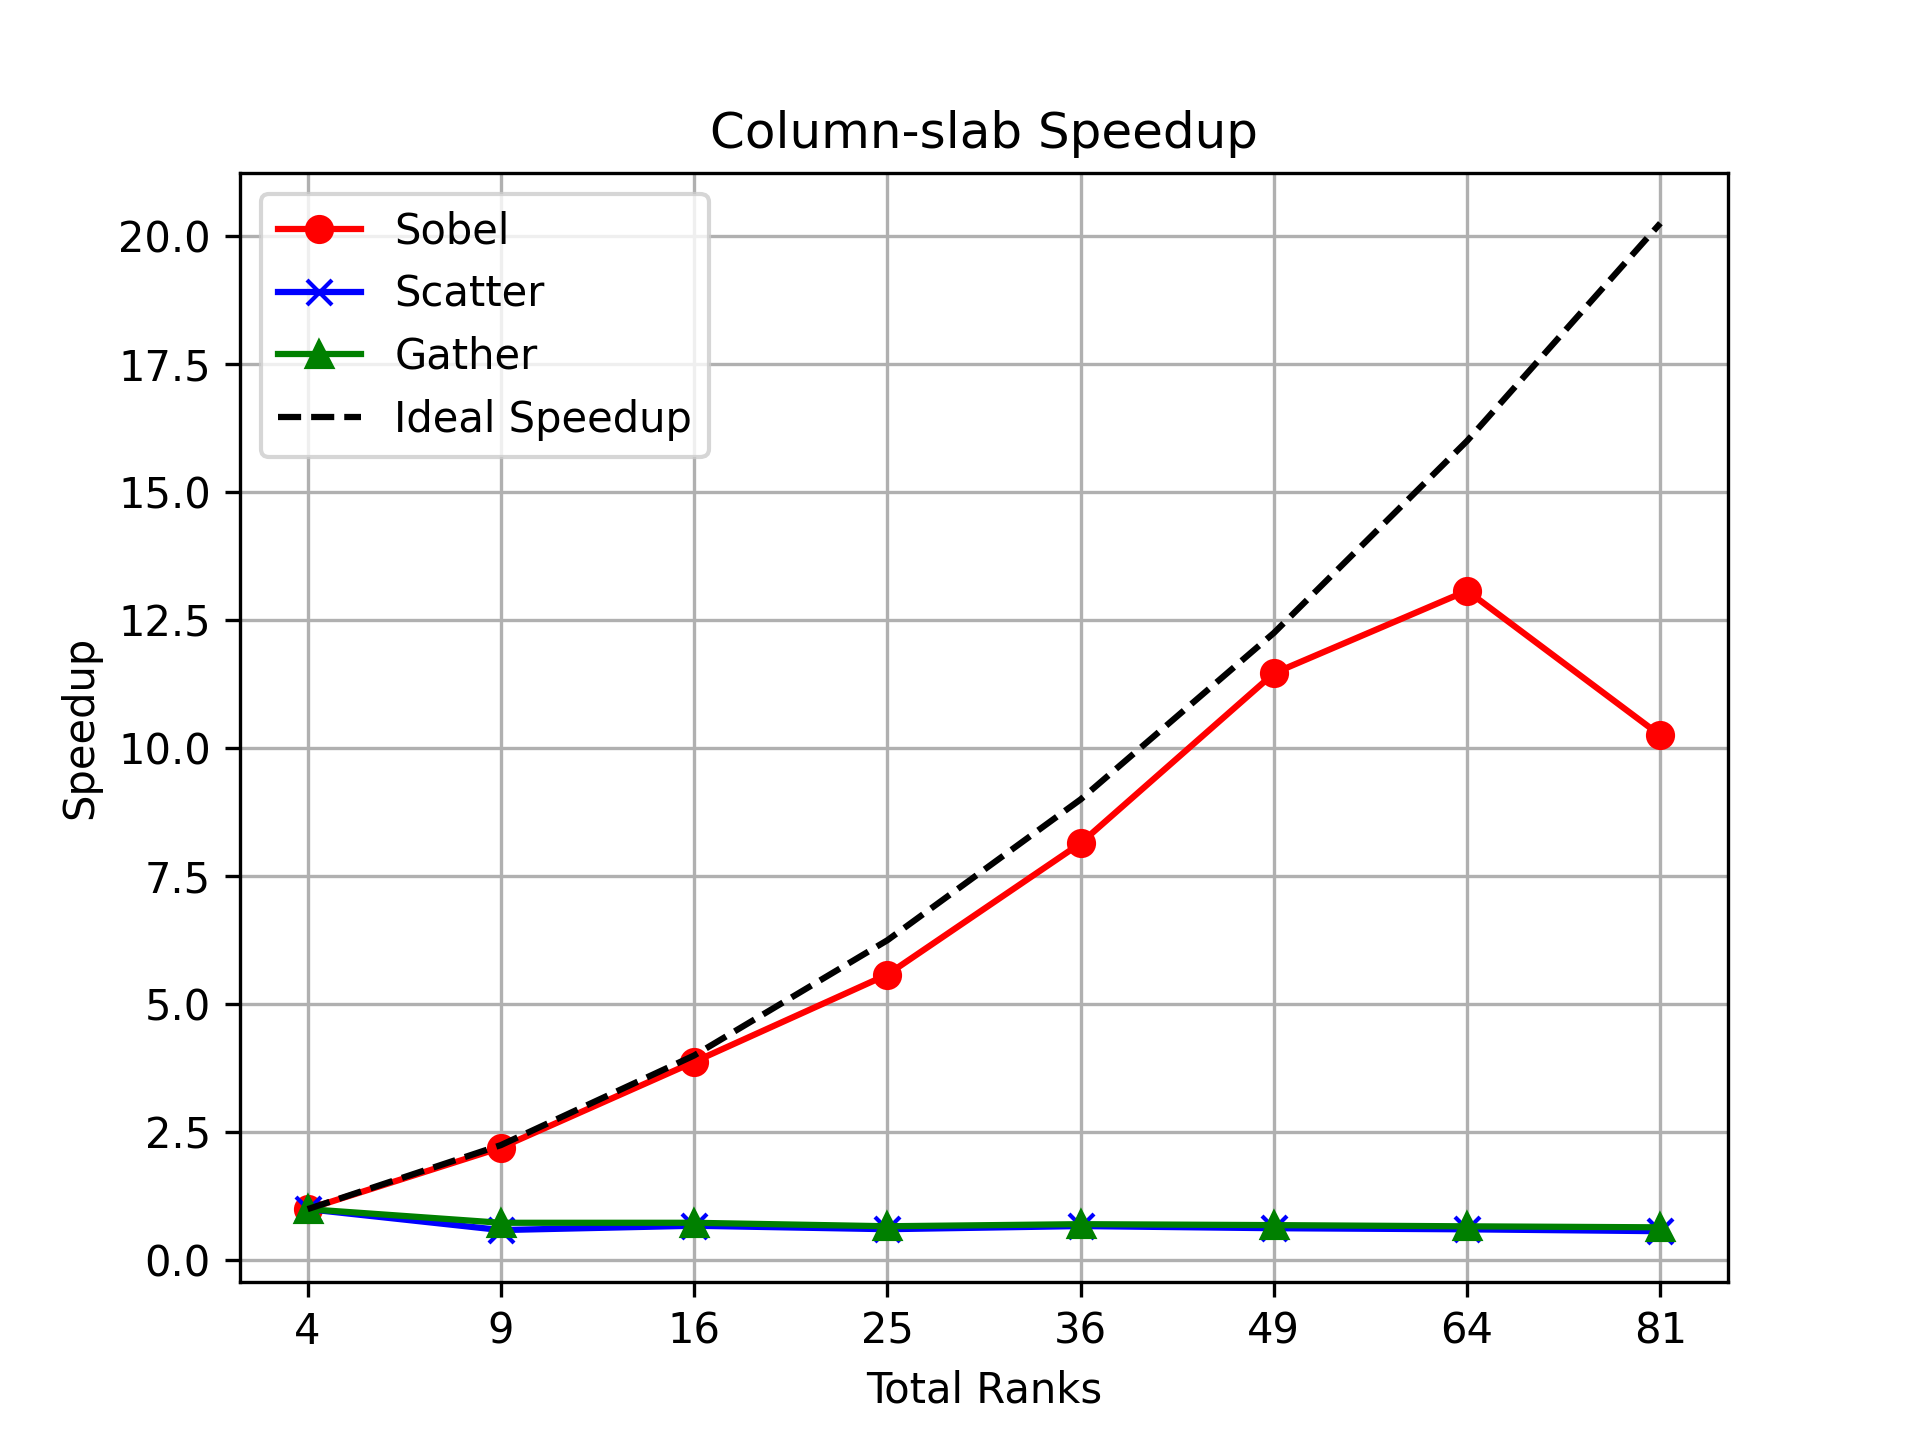
\includegraphics[width=1.0\linewidth]{images/column-slab_speedup.png}
    \caption{Speedup chart for Column-slab decomposition.}
    \label{fig:speedup-column}
\end{figure}

\begin{figure}[htbp]
    \centering
    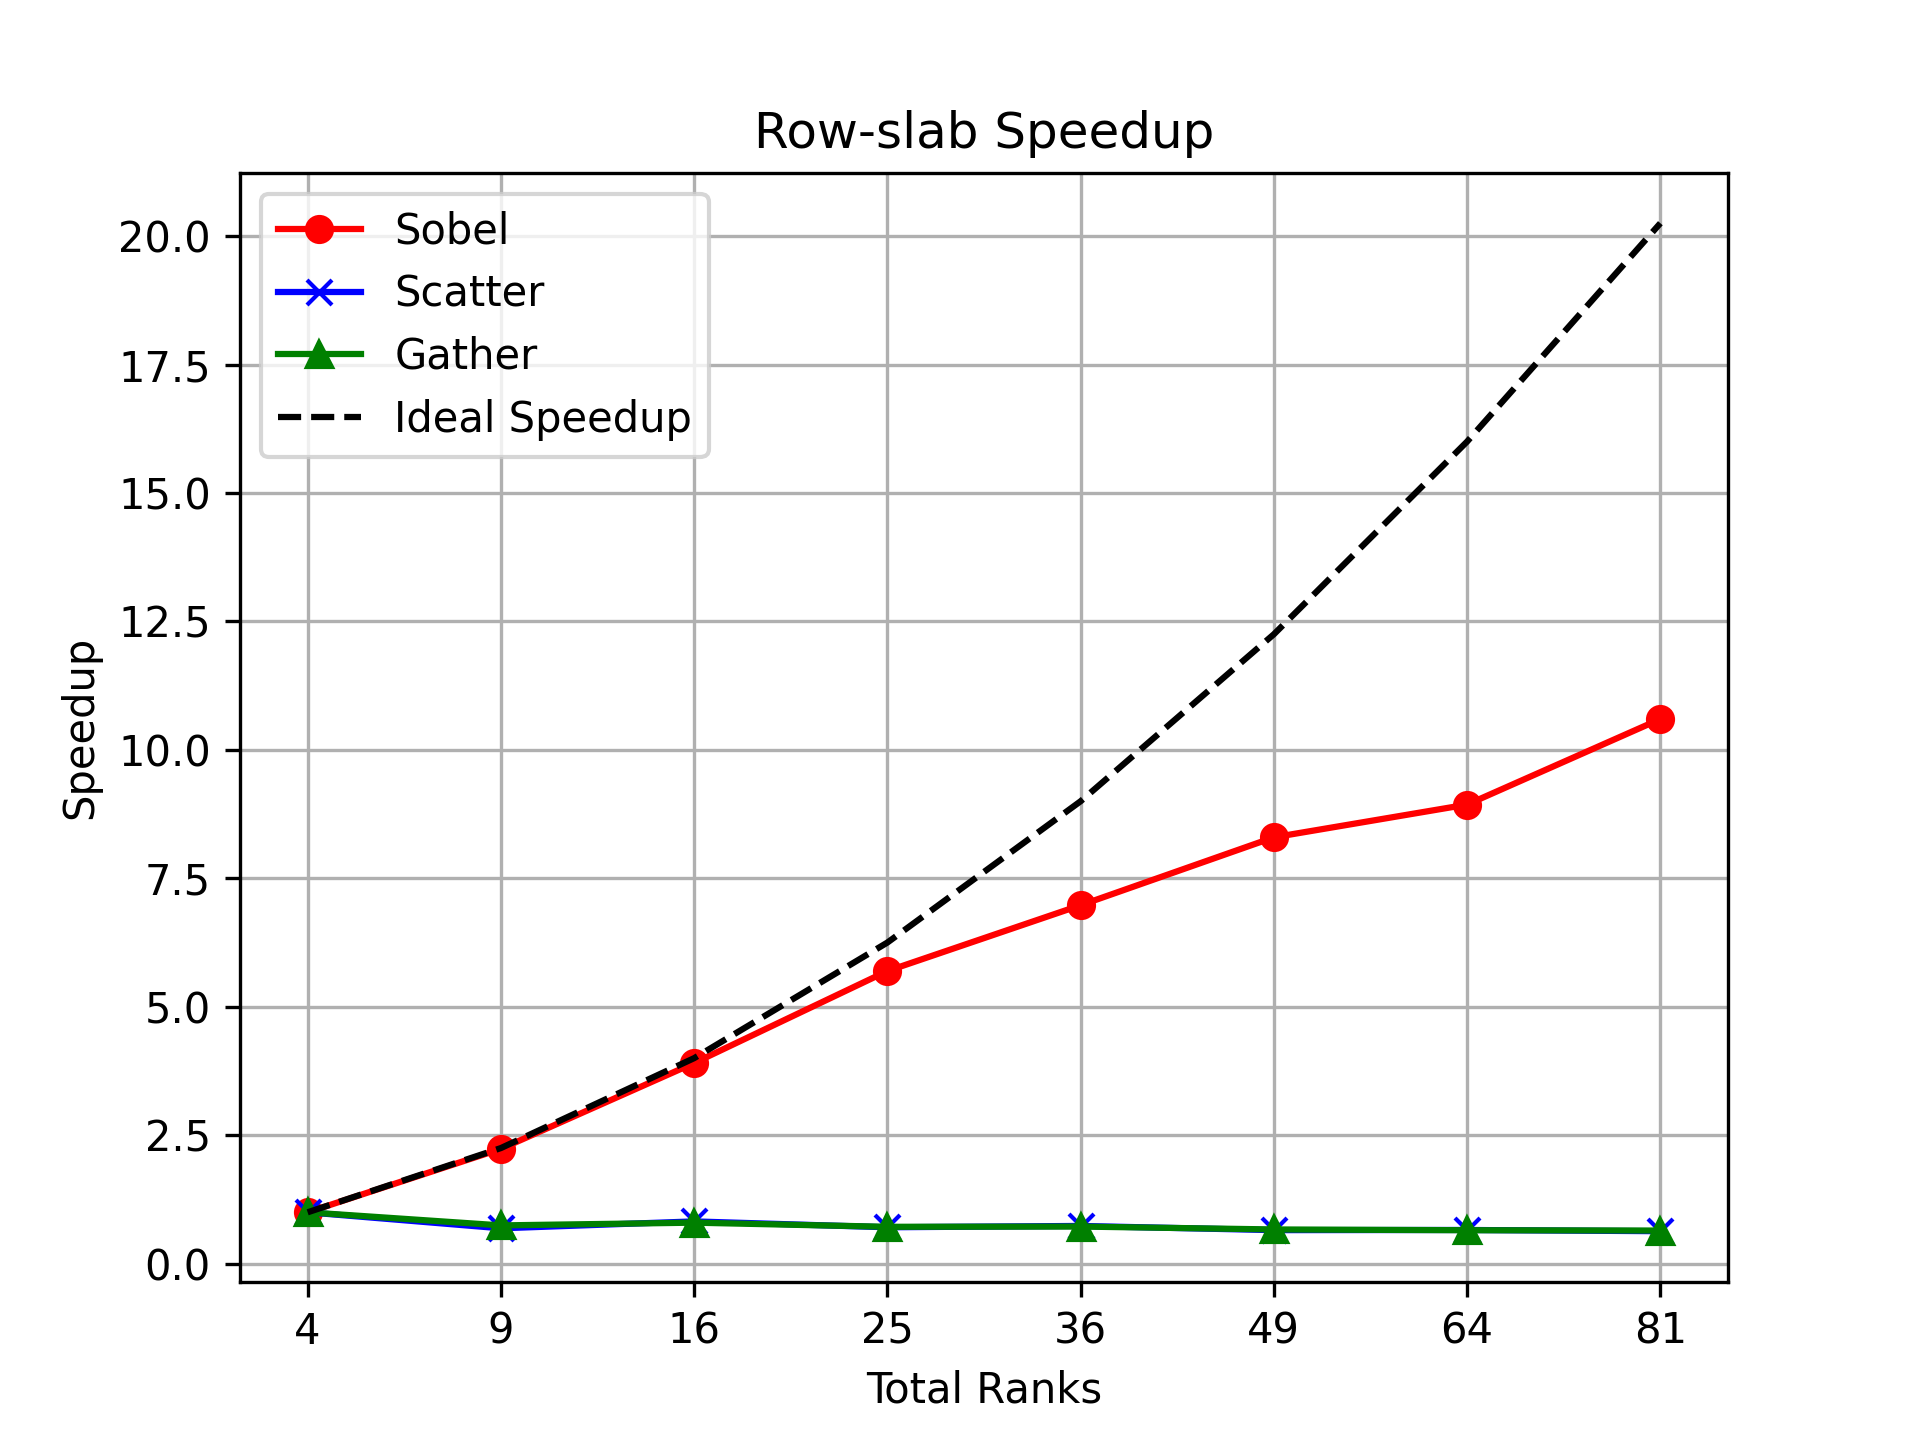
\includegraphics[width=1.0\linewidth]{images/row-slab_speedup.png}
    \caption{Speedup chart for Row-slab decomposition.}
    \label{fig:speedup-row}
\end{figure}

\begin{figure}[htbp]
    \centering
    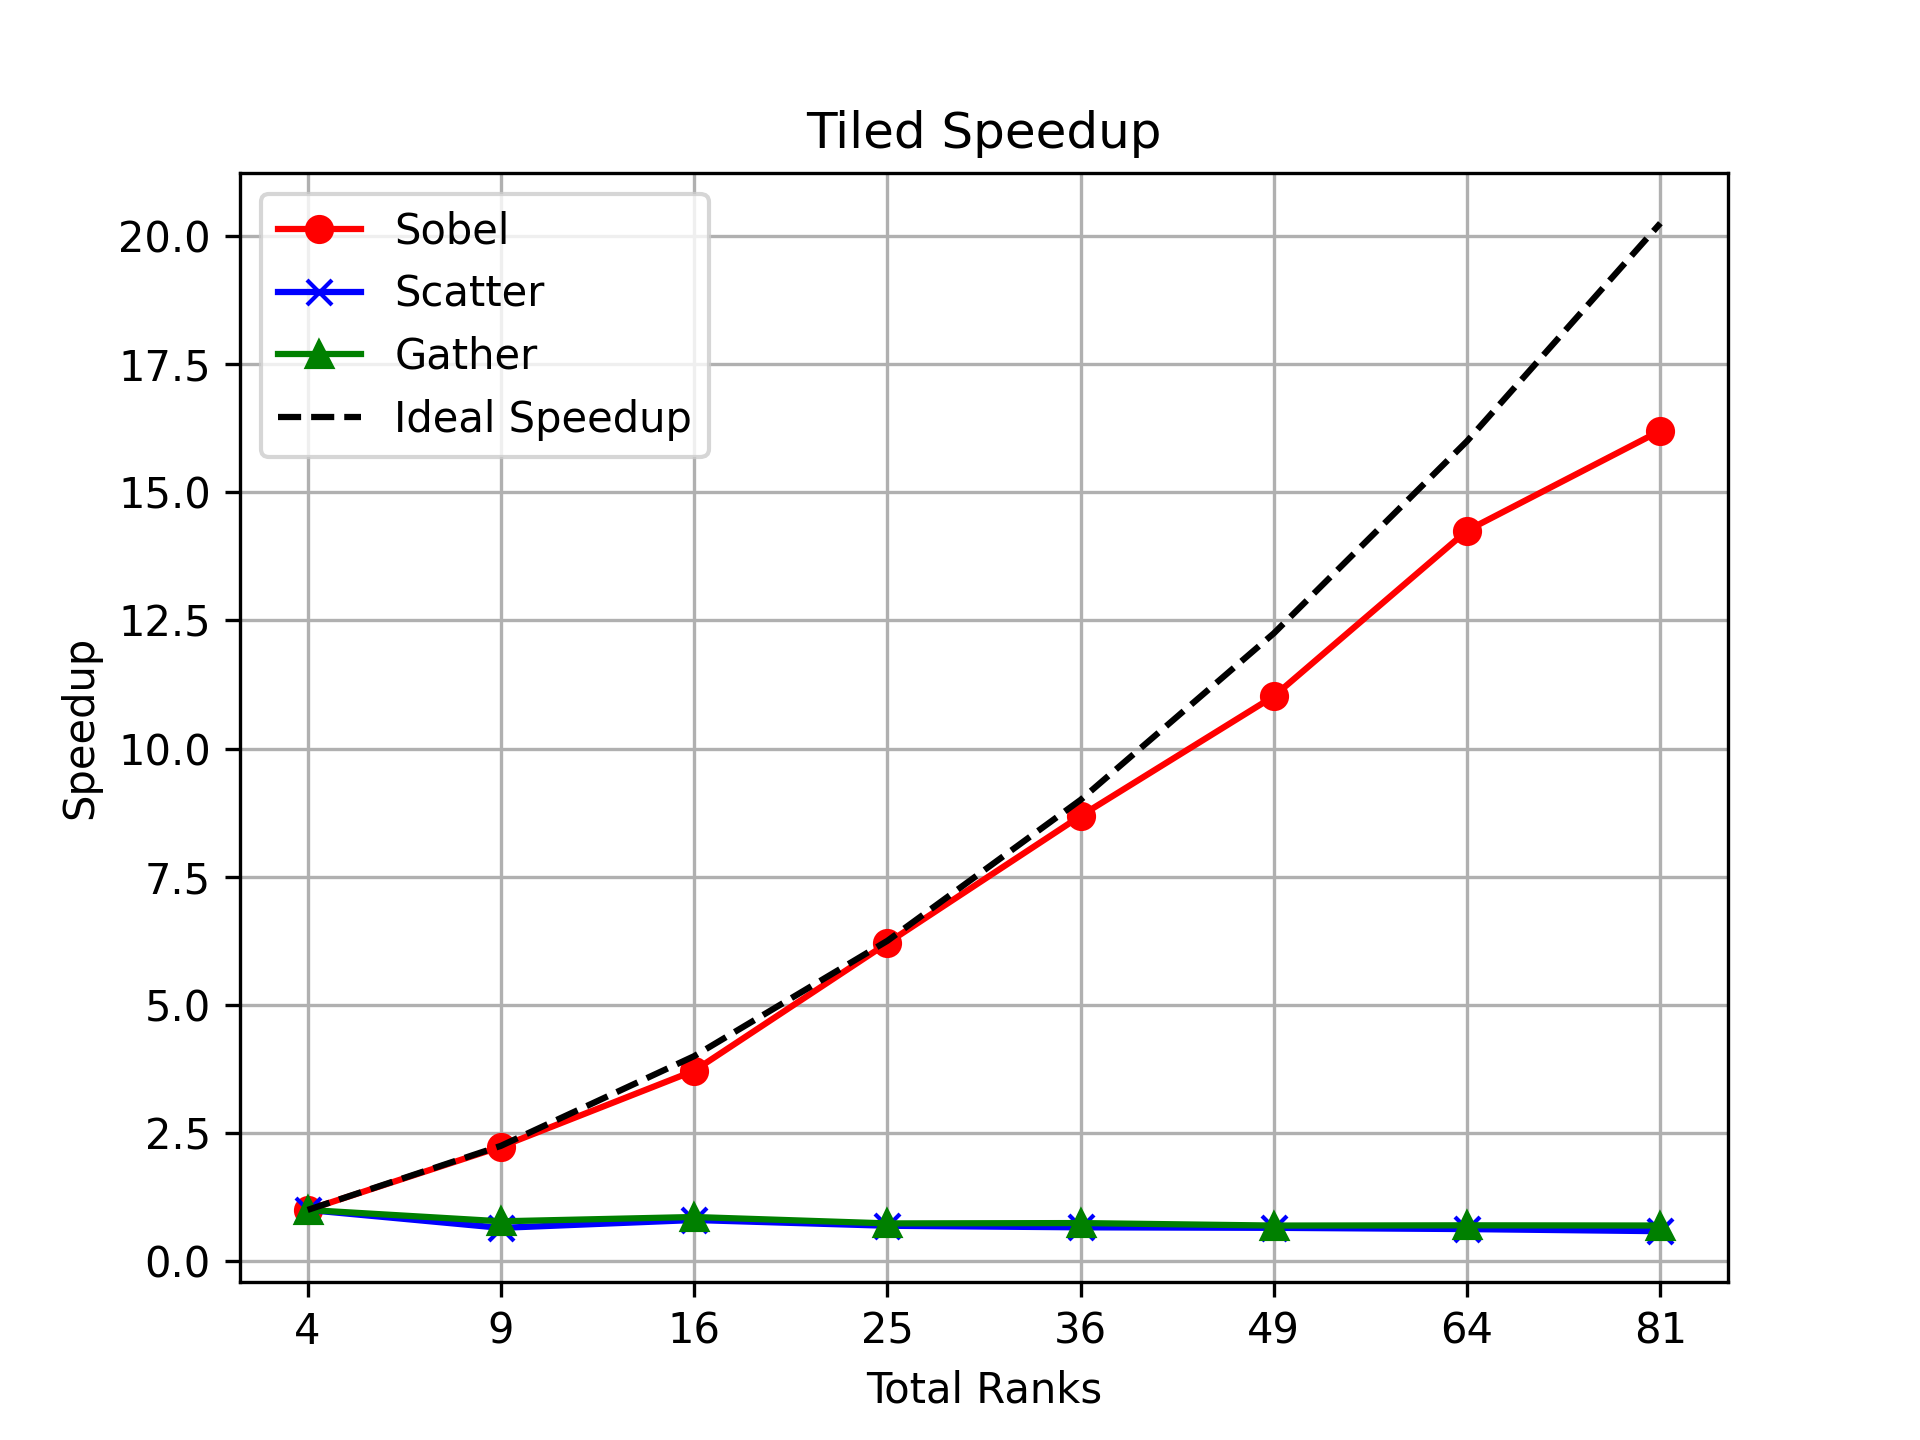
\includegraphics[width=1.0\linewidth]{images/tiled_speedup.png}
    \caption{Speedup chart for Tiled decomposition.}
    \label{fig:speedup-tiled}
\end{figure}

In this section, we analyze the runtime performance of the Sobel filter using three grid decomposition strategies: Column-slab, Row-slab, and Tiled decomposition. The speedup charts for these strategies, shown in Figures~\ref{fig:speedup-column},~\ref{fig:speedup-row}, and~\ref{fig:speedup-tiled}, illustrate the speedup of runtimes for the three computational stages: scatter, process, and gather. Below, we describe the observed performance characteristics for each strategy and discuss the underlying reasons.

As shown in Figure~\ref{fig:speedup-column}, the Column-slab decomposition achieved consistent speedup up to a total rank of 49, nearing ideal performance. However, the speedup gains plateaued at a total rank of 64, and a performance degradation was observed at a total rank of 81.

In contrast, as illustrated in Figure~\ref{fig:speedup-row}, the Row-slab decomposition showed consistent speedup with increasing total ranks, although it began to deviate slightly from ideal performance starting at a total rank of 36.

As shown in Figure~\ref{fig:speedup-tiled}, the Tiled decomposition consistently achieved near-ideal speedup, maintaining strong performance up to a total rank of 64. Unlike the Column-slab, it did not exhibit performance degradation at higher ranks.

The performance behavior of the Column-slab decomposition was initially expected to outperform the others due to its narrower tile width, which enhances cache efficiency when transitioning between rows. While it did show better speedup than Row-slab for lower ranks, the unexpected performance drop at a total rank of 81 may be attributed to inherent load imbalances. For instance, as shown in Table~\ref{tab:last-grid-sizes} and \ref{tab:last-grid-sizes}, the base grid size for 64 ranks is \(111 \times 5146\), with a last tile size of \(119 \times 5146\). In contrast, the base grid size for 81 ranks is \(87 \times 5146\), with a last tile size of \(152 \times 5146\). This disparity arises because the current implementation uses fixed dimensions for all tiles except the last one, causing the last tile to be disproportionately larger. This imbalance likely limited overall performance. To address this, a more balanced tile computation scheme should be implemented to ensure uniform tile sizes.

The superior performance of the Tiled decomposition is likely due to its more evenly distributed tile sizes, which mitigate the impact of slower ranks on runtime. As the runtime is ultimately constrained by the slowest rank, reducing disparities in tile sizes directly improves performance.

\begin{table}
    \centering
    \begin{tabular}{c|c|c|c}
        \textbf{Rank} & \textbf{Column-slab} & \textbf{Row-slab} & \textbf{Tiled} \\
        \hline
        4  & 1778 x 5146& 7112 x 1286& 3556 x 2573\\
        9  & 790 x 5146& 7112 x 571& 2370 x 1715\\
        16 & 444 x 5146& 7112 x 321& 1778 x 1286\\
        25 & 284 x 5146& 7112 x 205& 1422 x 1029\\
        36 & 197 x 5146& 7112 x 142& 1185 x 857\\
        49 & 145 x 5146& 7112 x 105& 1016 x 735\\
        64 & 111 x 5146& 7112 x 80& 889 x 643\\
        81 & 87 x 5146& 7112 x 63& 790 x 571\\
    \end{tabular}
    \caption{Base grid size of the tile for each decomposition method.}
    \label{tab:base-grid-sizes}
\end{table}

\begin{table}
    \centering
    \begin{tabular}{c|c|c|c}
        \textbf{Rank} & \textbf{Column-slab} & \textbf{Row-slab} & \textbf{Tiled} \\
        \hline
        4  & 1778 x 5146& \(7112 \times 1288\) & \(3556 \times 2573\) \\
        9  & 792 x 5146& \(7112 \times 578\)  & \(2372 \times 1716\) \\
        16 & 452 x 5146& \(7112 \times 331\)  & \(1778 \times 1288\) \\
        25 & 296 x 5146& \(7112 \times 226\)  & \(1424 \times 1030\) \\
        36 & 217 x 5146& \(7112 \times 176\)  & \(1187 \times 861\)  \\
        49 & 152 x 5146& \(7112 \times 106\)  & \(1016 \times 736\)  \\
        64 & 119 x 5146& \(7112 \times 106\)  & \(889 \times 645\)   \\
        81 & 152 x 5146& \(7112 \times 106\)  & \(792 \times 578\)   \\
    \end{tabular}
    \caption{Grid size of the last tile for each decomposition method.}
    \label{tab:last-grid-sizes}
\end{table}


The scatter and gather runtimes exhibited similar performance across all decomposition strategies. While their speedup dropped by approximately 30\% when increasing the total rank from 4 to 9, the performance stabilized for higher ranks. This consistency can be attributed to the use of subarray datatypes, which optimize communication by transforming data before transmission. By sending subregions of data in a single operation instead of row-by-row transfers, the number of communication events between ranks is minimized, leading to nearly identical scatter and gather performance across all methods.